\newcolumntype{C}[1]{>{\centering\arraybackslash}p{#1}}

\section{Ryšio mažame lauke technologija}

\subsection{Radio dažnio identifikavimo technologija}
Radio dažnio identifikavimo (angl. \textit{Radio-frequency identification}) (toliau- RFID) tai viena iš bevielio komunikavimo technologijų, kuri yra paremta elektromagnetinių bangų spektro dažniais, kurie padeda identifikuoti unikalius objektus. Pirmieji RFID panaudojo Britų armijos karininkai Antrajame pasauliniame kare, jie šią technologiją naudojo identifikuoti armijai priklausančius objektus, t.y. lėktuvus, radarus ir kt. \cite{Motlagh2012}. RFID sukuria vienos krypties arba dvikryptį bevielį duomenų srautą. Duomenų perdavime dalyvauja 2 aktoriai - žyma (angl. \textit{tag}), ir skaitytuvas (angl. \textit{reader} \cite{Igoe2014}. Skaitytuvas inicijuoja komunikavimą sukurdamas elektromagnetinio lauko bangas ir laukia atsakymo iš žymos. Žyma priima skaitytuvo komunikavimo užklausą ir grąžina rezultatą. Žemiau pateiktoje diagramoje (žiūrėti 2 pav.) pavaizduota RFID sistemą, šia sistemą bei daugelį kitų RFID sistemų sudaro šie 3 pagrindiniai komponentai \cite{Hunt2006}: 
\begin{enumerate}
    \item \textbf{Žyma}, taip pat dar vadinama - siųstuvu. Žyma yra sudaryta iš semikonduktoriaus mikroschemos, antenos. Taip pat kartais žyma turi vidinį maitinimo šaltinį - bateriją.
    \item \textbf{Skaitytuvas}, jis yra sudarytas iš antenos, radio bangų dažnių modulio siųsti ir gauti signalus iš žymos ir valdymo modulio.
    \item \textbf{Valdiklis} (angl. \textit{controller}), tiap pat dar vadinamas pagrindiniu kompiuteriu (angl. \textit{host}). Dažniausiai tai yra kompiuteris, kuriame yra duomenų bazė ir valdymo programinė įranga.
\end{enumerate}

\begin{figure}[H]
    \centering
    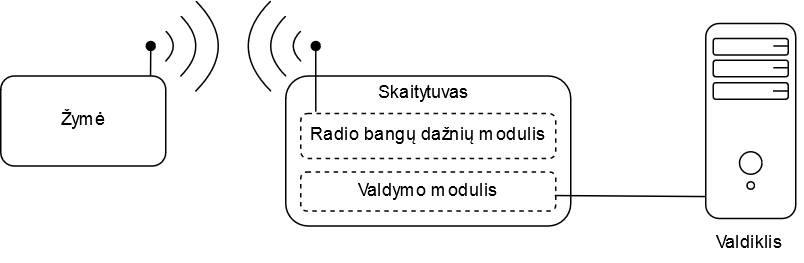
\includegraphics[scale=0.45]{images/RFID}
    \caption{RFID sistemos komponentų diagrama} 
\end{figure}

RFID žymos yra skirstomos į 2 tipus \cite{Igoe2014}:
\begin{enumerate}
    \item Aktyvus komunikavimo tipas. Šiam tipui priklauso tos RFID technologijos, kurių aktoriai turi savo nuosavus energijos šaltinius. Kuomet adresatas siunčia rezultatą iniciatoriui, jis naudoja energiją, kuri yra gaunama iš nuosavo maitinimo šaltinio.
    \item Pasyvus komunikavimo tipas. Šiam tipui priklauso tos RFID technologijos, kurių vienas iš adresatų neturi nuosavo energijos šaltinio, t.y. adresatas, o kitas turi. Tam, kad adresatas išsiųstų rezultatą, jis reikiamą energiją gauną iš iniciatoriaus sukurto magnetinio lauko.
\end{enumerate}
Lentelėje (žiūrėti 2 lentelę) pateikiamas aktyvios ir pasyvius žymos palyginimas.

\begin{table}[!ht]
    \centering
    \renewcommand{\arraystretch}{1,2}
    \begin{tabular}{| p{10em} | p{12em} | p{12em} |}\hline
        \backslashbox[10em]{Ypatybės}{Tipai}
        &\makebox[12em]{Aktyvus}&\makebox[12em]{Aktyvus}\\\hline
        Matinimo šaltinis & Vidinis & Išorinis\\\hline
        Skaitymo diapazonas & Didelis - iki 100 metrų & Nėra didelis - iki 3 metrų   \\\hline
        Žymos veikimo laikas & Kadangi žyma turi vidinį maitinimo šaltinį, jis nuolatos būna veikimo būsenoje & Žyma pradeda veikti tik tuomet, kai skaitytuvas inicijuoja komunikavimą \\\hline
        Magnetinio lauko stiprumas & Magnetinis laukas nėra stiprus, nes žyma naudoja vidinę energiją tam, kad išsiųstų signalą  & Sukuriamas stiprus magnetinis laukas, nes šio magnetinio lauko dėka, žyma įgyja energijos išsiųsti signalą \\\hline
        Naudojimo terminas & Naudojomi terminas priklauso nuo maitinimo šaltinio galiojimo termino & Naudojimo terminas nėra apibrėžtas \\\hline
        Saugomų duomenų dydis &  Didesnis, dažnu atvėju 128 kilobaitai (angl \textit{Kilobyte}) & Mažas, dažniausiai 128 baitai (angl. \textit{Byte})  \\\hline
        Dydis & Dydis priklauso nuo matinimo šaltinio dydžio & Mažas \\\hline
        Kaina & Brangesnis nei pasyvus & Brangesnis nei aktyvus \\\hline
    \end{tabular}
    \caption{Aktyvios ir pasyvios RFID žymos palyginimas}
\end{table}

RFID technologijos charakteristikos nėra pastovios, šios technologijos savybėm didžiausią įtaką daro parinktas elektromagnetinės bangos dažnis, kuris yra naudojamas komunikavimui tarp skaitytuvo ir žymos, todėl kuriant sistemą, kuri yra paremta RFID technologija, svarbu pasirinkti tinkamą bangos dažnį. RFID technologijos naudojami elektromagnetinių bangų dažniai - kilometrinės bangos žemieji dažniai (toliau - ŽD), dekametrinės bangos aukštieji dažniai  (toliau - AD), decimetrinės bangos ultra aukšti dažniai (toliau - UAD) ir mikrobangų dažniai. Šių dažnių naudojimą RFID sistemose aprašo ISO ir IEC standartai. Elektromangnetinių bangų dažniai daro įtaką šioms RFID savybės \cite{Hunt2006}:
\begin{enumerate}
    \item \textbf{Skaitymo diapazonas}. Žemesnių bangų dažnių RFID skaitymo diapozonas buna mažas. Aukštesnių bangų dažnių RFID skaitymo diapozonas yra didesnis, ypač jeigu naudojamas aktyvus RFID tipas.
    \item \textbf{Aktyvus ir pasyvus RFID}. Istoriškai, pasyvus RFID naudodavo ŽD ir AD dažnius, o aktyvus - UAD ir mikrobangų dažnius, tačiau šiuo metu abiejų tipų RFID gali naudotis aukštesnis dažnius, t.y. UAD ir mikrobangų dažnius.
    \item \textbf{Radijo dažnių trukdžiai}. Žemesnių dažnių RFID yra labiau atsparūs interferencijai, nei aukštesnių dažnių RFID.
    \item \textbf{Vandens ir metalo įtaka}. Mikrobangos ir UAD turi didesnę tikimybę būti sugertiems skysčio, todėl šių dažnių RFID nėra tinkamas naudoti šlapiem objektam. Kandagi metalas atspindi elektromagnetines bangas, jos negali prasiskverbti pro jį, tačiau net šalia esantis metalas taip pat gali atspindėti elektromagnetines bangas, todėl tiek aukštesnio dažnio, tiek žemesnio dažnio bangoms metalas daro įtaką. Žemesnio dažnio bangos yra paveikiamos metalo mažiau nei aukštesnio.
\end{enumerate}
Žemiau pavaizduotoje lentelėje (žiūrėti 3 lentelę), pateikiamos RFID tipų naudojami elektromagnetiniai bangų dažniai, jų naudojimą apibrėžiantys standartai\cite{Caglar2016}.

\begin{table}[!ht]
    \centering
    \renewcommand{\arraystretch}{1,2}
    \begin{tabular}{m{10em}m{10em}m{10em}m{10em}} 
        \hline
        Elektromagnetinė banga            & Bangos dažniai    & RFID tipas    &Standartai   \\ 
        \hline
        ŽD                     & 125-134.2 KHz & Pasyvus & ISO 11784 \par ISO/IEC 18000-2A \par ISO/IEC 18000-2B   \\ 
        \hline
        AD                     & 13.56 MHz & Pasyvus  &  ISO 18000-3 \par ISO/IEC 15693 \\ 
        \hline
        \multirow{2}{*}{UAD} & 433 MHz       & Aktyvus   &  ISO 18000-7    \\ 
        \cline{2-4}
                                & 860 ir 915 MHz      &  Pasyvus ir Aktyvus  &  ISO 18000-6A \par ISO 18000-6B \par ISO 18000-6C    \\ 
        \hline
        Mikrobangos                       & 2.45 ir 5.8 GHz         & Pasyvus ir Aktyvus &  ISO 18000-4  \\
        \hline
    \end{tabular}
    \caption{Aktyvaus ir pasyvaus RFID komunikavimo tipų palyginimas}
\end{table}

\subsection{Ryšio mažame lauke}
\subsubsection{Sąvoka}
NFC tai bevielo komunikavimo technologija, šis technologija yra pagrįsta anksčiau minėtos RFID technologijos standartais ir interfeisais, todėl įrenginiai, kurie paremti NFC technologija, gali komunikuoti su dauguma RFID technologijos irenginių \cite{Motlagh2012}. NFC įrenginiai tarpusavyje komunikuoja 13.56 MHz elektromagnetinių bangų dažniu, duomenų perdavimo greitis svyruoja nuo 106 kilobitu per sekundę iki 424 kilobitų per sekundę \cite{whitepapaer}. Maksimalus veikimo atsumas tarp NFC įrenginių literatūroje minimas ne vienodas, apibendrinus literatūros šaltinius, maksimalus veikimo atstumas yra tarp 4 centimetrų ir 20 centimetrų \cite{whitepapaer} \cite{Motlagh2012} \cite{Leora1980}. Pagrindiniai skirtumai tarp RFID ir NFC technologijų \cite{Leora1980}:
\begin{enumerate}
    \item Komunikavimo atvėju, atstumas tarp NFC įrenginių turi būti mažas, o RFID technologijoje naudojant aktyvias žymes, atstumas gali būti žymiai didesnis.
    \item NFC technologijoje naudojamos tik pasyvios žymės, o RFID technologijoje naudojomos tiek aktyvios, tiek pasyvios žymės.
    \item Dėl to, kad komunikavimo atsumtas yra mažas, duomenų perdavimas laikomas saugesniu nei RFID.
    \item Dėl to, kad komunikavimo atstumas yra mazas, skaitytuvas komunikuoja su norima žyma, mažėja tikimybė jog skaitytuvo veikimo lauke yra keletas žymų.
\end{enumerate}
 

\subsubsection{Duomenų apsikeitimo specifikacija}
NFC duomenų apsikeitimo formatas (angl. \textit{NFC Data Exchange Format}) (toliau - NDEF) tai standartas, kuris nusako duomenų apsikeitimo formatą tarp NFC įrenginio ir NFC žymės arba tarp dviejų NFC įrenginių \cite{Leora1980}. Komunikavimo metu, siunčiama NDEF žinutė, kurią sudaro vienas arba daugiau NDEF įrašų (angl. \textit{records})(žiūrėti 3 pav.) . NDEF įrašą sudaro antraštė (angl. \textit{header}) ir informacija (angl. \textit{payload}), kurios dydis yra iki 2\textup{32}-1 baitų \cite{NFCForum2006}. Norint talpinti didesnį kiekį duomenų, NDEF įrašai gali būti apjungti. Kadangi NDEF žinutę gali sudaryti daugiau nei vienas įrašas, svarbu indikuoti žinutės rėžius, todėl pirmasis įrašas žinutės eilėje turi žinutės pradžios indikatorių, o paskutinis įrašas - žinutės pabaigos indikatorių.

\begin{figure}[H]
    \centering
    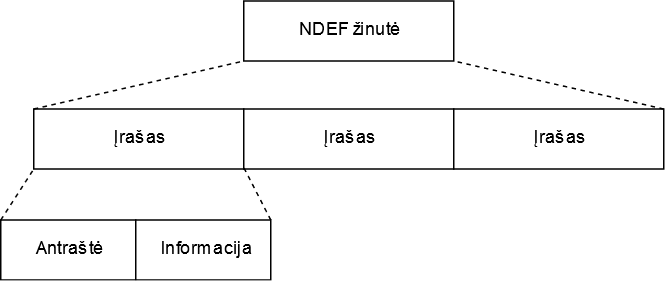
\includegraphics[scale=0.5]{images/NDEF}
    \caption{NDEF žinutės sudedamosios dalys} 
\end{figure}


Žemiau pateiktoje lentelėje (žiūrėti 4 lentelę) yra nurodoma NDEF žinutės įrašą sudarantys laukai. Žinutės įrašą sudaro 12 laukų, iš kuriu 11 sudaro įrašo antraštę, o 1 sudaro informaciją.
Antraštės laukai yra šie \cite{NFCForum2006}: 
\begin{itemize}
    \item \textbf{ŽPR}, Žinutės pradžios indikatorius (angl. \textit{Message begin}), šis laukas yra 1 bito dydžio ir jis nurodo žinutės pradžią.
    \item \textbf{ŽPB}, Žinutės pabagiso indikatorius (angl. \textit{Message end}), šis laukas yra 1 bito dydžio ir jis nurodo žinutės pabaigą.
    \item \textbf{DD}, Duomenų dalis (angl. \textit{Chunk flag}), šis lukas yra 1 bito dydžio ir nurodo, ar įrašo informacija yra pilna, ar įraše laikoma informacija yra tik dalis pilnos siunčiamos informacijos.
    \item \textbf{TĮ}, Trumpas įrašas (angl. \textit{Short record}), šis laukas yra 1 bito dydžio, jis norodo ar informacijos kiekis yra mažesnis nei 2\textup{8}-1 baitai.
    \item \textbf{IB}, ID būvimas (angl. \textit{ID length present}), šis laukas yra 1 bito dydžio, jis nurodo ar įraše yra saugomas ID.
    \item \textbf{ĮTF}, Įrašo tipo formatas (angl. \textit{Type name format}), šis laukas yra 3 bitų dydžio, jis nurodo kokio formato yra NDEF įrašo tipas. Tipo formatų sarašas yra pateiktas literatūroje \cite{Leora1980}.
    \item \textbf{Įrašo tipo dydis} (angl. \textit{Type length}), šis laukas yra 1 baito dydžio, jis nurodo koks yra įrašo tipo lauko dydis.
    \item \textbf{ID dydis} (angl. \textit{ID length}), šis laukas yra 1 baito dydžio, jis yra saugomas įraše tuomet, kai IB lauko bitas yra 1. Šis laukas nurodo koks yra ID lauko dydis.
    \item \textbf{Informacijos dydis} (angl \textit{Payload length}), šio lauko dydį nusako TĮ lauko reikšmė. Jeigu TĮ lauko bitas yra 1, tuomet Informacijos dydžio lauko dydis yra 1 baitas. Jeigu TĮ lauko bitas yra 0, tuomet Informacijos dydžio lauko dydis yra 4 baitai.
    \item \textbf{Įrašo tipas} (angl. \textit{Type}), šis lauko dydi nusako Įrašo tipo dydžio laukas. Šis laukas nurodo įrašo informacijos lauko tipą. Įrašo tipas turi būti pateiktas tokiu formatu, kuris yra nurodomas ĮTF lauke.
    \item \textbf{ID}, šio lauko dydį nusako ID dydžio laukas. Šis laukas nurodo įrašo unikalų identifikatorių.
\end{itemize}
Informacijos lauko dydį NDEF įraše nusako antraštės informacijos dydžio laukas. Šiame lauke yra saugoma informacija, kuria yra keičiamasis tarp NFC įrenginių.

\begin{table}[!ht]
    \centering
    \renewcommand{\arraystretch}{1,7}
    \begin{tabular}{C{2em}C{2em}C{2em}C{2em}C{2em}C{2em}C{2em}C{2em}l}
        7                         & 6                        & 5                       & 4                       & 3                       & 2 & 1 & 0                 &                        \\ 
        \hline
        \multicolumn{1}{|c|}{ŽPR} & \multicolumn{1}{c|}{ŽPA} & \multicolumn{1}{c|}{DD} & \multicolumn{1}{c|}{TĮ} & \multicolumn{1}{c|}{IB} & \multicolumn{3}{c|}{ĮTF } & \parbox[t]{2mm}{\multirow{6}{*}{\rotatebox[origin=c]{270}{Antraštė}}}  \\ 
        \cline{1-8}
        \multicolumn{8}{|c|}{Įrašo tipo dydis}                                                                                                                         &                        \\ 
        \cline{1-8}
        \multicolumn{8}{|c|}{Informacijos dydis}                                                                                                                       &                        \\ 
        \cline{1-8}
        \multicolumn{8}{|c|}{ID dydis}                                                                                                                                 &                        \\ 
        \cline{1-8}
        \multicolumn{8}{|c|}{Įrašo tipas}                                                                                                                              &                        \\ 
        \cline{1-8}
        \multicolumn{8}{|c|}{ID}                                                                                                                                       &                        \\ 
        \hline
        \multicolumn{8}{|c|}{}                                                                                                                                         &                        \\
        \multicolumn{8}{|c|}{Informacija}                                                                                                                              &                        \\
        \multicolumn{8}{|c|}{}                                                                                                                                         &                        \\
        \cline{1-8}
    \end{tabular}
    \caption{NDEF žinutės įrašas \cite{NFCForum2006} }
\end{table}
% \subsection{NFC techologijos dabartis ateitis} ???
% \subsection{NFC technologijos palyginimas} ???